\section{Introduction}
Tax collection has repeatedly been shown to be crucial for state development \citep{besley2014developing}. In this context, value-added tax (VAT) has been proven to be an effective tool to raise revenues \citep{keen2006vat}. The VAT systems across the world are, however, afflicted with size-dependent regulations. Such policies form an elementary part of the VAT administration across countries, with both the VAT registration thresholds and the VAT reporting frequency thresholds being dependent on the reported firm revenue.

\todo[inline, caption={Liquidity concerns}]{In the public version, we have to talk about liquidity.}
\todo[inline, caption={Optimal literature}]{What does the literature say? Anyway for us to say, econ 101 says that this should not matter}
However, the benefit of such size-dependent regulations to the tax authority is unclear. First, the tax authority may prefer to receive as much information as fast as possible. Second, the government might be liquidity constrained, so that it also prefers to receive the VAT payments from the firms at as high frequency as possible. On the other hand, the literature has provided theoretical arguments that the government should economize on administrative and compliance costs by exempting small firms from taxation \citep{dharmapala2011tax}. Such optimizing concern might be even more important for low- and middle- income countries, where compliance costs are of first order concern. Indeed,  compliance costs, relative to firm size, might be greater for smaller companies - with little benefit to the tax authority \citep{internationaltaxdialogue2007,internationaltaxdialogue2013}. In the context of many countries, firms close to the VAT registration threshold actively manipulate their reported revenues in order to avoid registering for VAT \citep{onji2009response,gebresilasse2016firm,liu2017vat,harju2016effects, boonzaaier2017small}. Furthermore, recent work has shown that firms also respond to the VAT filing or the so-called administrative thresholds \citep{asatryan2017responses}. 
\todo[inline, caption={Reframe Armenia paper}]{We have to be careful about how we talk about armenia paper. In its current form it is not clear how we are different from it.}

In this paper, we use an administrative dataset from the state of Delhi in India to first show that a policy which mandated different frequencies of filing based on reported turnover resulted in bunching of firms below the thresholds at all levels. Using the change in these reporting policies, we provide further evidence that such sharp bunching indeed occurs due to the VAT reporting frequency thresholds. Second, we calculate the VAT revenue losses due to such bunching and document the longer-term impact of the VAT reporting frequency thresholds. Finally, the subsequent withdrawal of the policy allows us to show that in a regime with size-dependent reporting requirements, more frequent reporting does not lead to greater levels of VAT collection.
\todo[inline, caption={Redo}]{The above paragraph is the replica of the abstract}

Our paper is the first, apart from \citet{asatryan2017responses}, to carefully investigate the firm responses to the VAT filing thresholds on the intensive margin. The unique setting in the state of Delhi in India allows us to simultaneously look at the firm responses at several different levels of thresholds. A careful analysis of the VAT filing thresholds fills an important gap in the literature: while the VAT registration thresholds are present in almost all countries with VAT administration, the VAT filing thresholds are also ubiquitous. 

Many countries have a uniform VAT reporting regulation on either a monthly (e.g., Argentina, India [GST]), or a bi-monthly (e.g., Barbados), or a quarterly (e.g., Cyprus) frequency. Moreover, there are many countries with policies that mandate frequency of VAT reporting based on firm size. Out of a 2015 sample of 103 countries for which we could determine with certainty, 39 countries size-dependent frequencies of VAT reporting and payments.\footnote{Based on survey of the data from \citet{ey2015worldwideguide}.} Among these there are both high-income (e.g., Austria, Germany, Denmark, Finland, France, Ireland, Spain, UK, etc.) as well as low- and middle-income (e.g., Botswana, Colombia, Mauritius, Philippines, South Africa, Swaziland) countries. If firms misreport their revenue in order to avoid filing (and remitting) VAT returns more frequently, it is important to understand the associated costs to the VAT collections. 
% * <shekhar.mittal@gmail.com> 2018-05-08T04:09:10.274Z:
% 
% Need to rephrase the above line.
% Why would a fiscally constrained government care? How does a greater frequency benefit that government?
% ^.
%Therefore, it is crucial to understand how firms respond to such size-dependent regulation more generally, and specifically to the VAT filing thresholds.

Before answering this question empirically, it is important to understand what is the optimal ``first-best'' policy with regards to VAT filing frequencies. A liquidity constrained government, which might be the case in  low- and middle-income countries, may prefer to receive the VAT reports and the associated payments with as high a frequency as possible. On the other hand, very high frequencies of VAT reporting and payments may  impose a significant burden on firms, especially on smaller ones. The trade-off is relatively clear: while the government prefers, for several reasons, to obtain information and the VAT payments as frequently as possible, it effectively subsidizes smaller firms - those, eligible for VAT - by imposing less stringent filing requirements on them. The problem occurs when such policies result in the firms actively avoiding filing more frequently, by either underreporting their actual revenues, or by under-producing and thus intentionally reducing their growth. Both of those channels are problematic: The first one creates an environment which via the choice of policies fosters a culture of evasion and avoidance, which is especially troublesome for the low- and middle-income countries. The second, underproduction channel, results in production inefficiencies, keeping the economy below its potential. In the paper, we provide a simple welfare analysis, by calculating the minimum compliance costs needed at the level of each of the reporting categories (annual, bi-annual, quarterly, and monthly) for the policy to be optimal, despite the revenue costs incurred by the tax authority. 
\todo[inline, caption={State the reasons}]{What are the reasons alluded to above?}
\todo[inline, caption={SM: Reason for relief to smaller firms}]{Empirically find out how much revenue is coming from the top firms.}


\todo[inline, caption={Policy of interest and results}]{New para: We have to describe the policy and the results}
The paper is organized as follows. The following section describes some of the related literature. \Cref{sec:background} describes the VAT system in Delhi, and describes the reforms in the VAT filing system. \Cref{sec:3-data} describes the administrative level data from Delhi that we use for our analysis. \Cref{sec:methodology} explains the methodology we use for the analysis. \Cref{sec:3-results} presents the results of our analysis of the firm response, of the revenue implications, and of welfare. \Cref{sec:3-conclusion} concludes.

\section{Related Literature
\label{sec:related-literature}}

We contribute to several strands of literature. Most generally, we build on the literature on the effects of size-dependent policies on firm behavior. The literature has shown extensively that such size-based regulations can and does lead to distortions \citep{gollin1995taxes,guner2008macroeconomic}. \citet{garicano2016firm} look at the context of labor laws in France, which start to bind firms with 50 or more employees. They find, using the administrative-level firm data, that the cost of such regulations is equivalent to a 2.3\% tax on labor, and that such regulations equal to welfare costs to the tune of 3.4\% of GDP. They also show that such size-dependent regulations are effectively subsidizing small firms, at the cost to workers and to some extent large firms. In the context of taxation, \citet{almunia2018under}, show that the threshold relevant for the large tax payers unit, which monitors large firms in Spain, results in strategic bunching of the firms in order to avoid stricter monitoring by the tax authority. Finally, they show that extending stricter monitoring to small businesses would generally generate substantial welfare gains.

Such size dependent policies are ubiquitous across countries. In their cross-country study, \citet{bachas2017size} for instance find that firm size has large effects on tax enforcement and the resulting tax compliance, with negative effects on giving bribes. Importantly for our work, they show that such a size gradient in tax enforcement is the strongest in developing countries. In the VAT context, \citet{mittal2017vat} show that strengthened paper trail leads to an increase in tax collection, primarily driven by the behavior of the largest firms. 

More specifically, we add on to the wide literature discussing the VAT policy, both theoretically and empirically. \citet{keen2006vat}, for instance, discuss the problematic aspects of the VAT policy in the EU countries, particularly when specific policy aspects result in a greater propensity for tax evasion and fraud. They also look at the possibility of a federal VAT system in the US. In their book, \citet{bird2007vat} discuss the application of VAT in lower income countries, and note the particularities pertaining to developing and transition countries. According to them, many problems occur when implementing VAT in most developing and transition countries, including flawed design such as inappropriate thresholds, as well as failures in implementation such as poor administrative procedures and insufficient audit.   

Additionally, we contribute to the literature on calculating the hassle costs affiliated with filing taxes. In this realm, \citet{benzarti2017taxing} estimates the cost of filing income taxes using US income tax return data. He finds that such hassle costs are increasing with income of households. 

We also add on to the literature on the specific literature analyzing the so-called VAT registration thresholds:
in those cases, firms below a certain size are exempt from registering for the VAT system and thus from paying 
VAT. In their theoretical work, \citet{keen2004optimal} look at the optimal registration threshold in the case of VAT, and show that such a threshold will necessarily lead to production inefficiencies via the bunching below the thresholds. 

A growing literature has empirically analyzed the effect of the VAT registration threshold. The first paper to recognize the reaction of firms to the VAT registration threshold was \citet{onji2009response}, which documents that large firms masquerade as many small firms in response to the VAT registration threshold in Japan. \citet{liu2017vat} theoretically and empirically consider the VAT registration notches and voluntary registration below the VAT registration threshold in the context of the UK. Their bunching estimates, based on separate annual observations of British firms between 2004 and 2010, are in the range between 0.815 and 1.286. They furthermore look at the determinants of voluntary registrations and of the bunching behavior, listing the low cost of inputs relative to sales, high proportion of business-to-customers sales, and high product market competition as determinants of higher bunching. \citet{harju2016effects} look at the impact of the VAT registration threshold on the behavior of small Finnish firms. They find that the firms actively avoid VAT liability, and that such avoidance is directly caused by the compliance costs of VAT. Furthermore, they find that the bunching behavior persists over the long-term, implying that the VAT registration threshold permanently hinders the growth of small firms. They find a strong bunching response to the VAT notch, of 3.63. 

In the context of a developing country, \citet{boonzaaier2017small} use tax register data from South Africa to look at the effects of several discontinuities in the tax schedule on the behavior of small firms. Among other discontinuities, their work also looks at the VAT registration notch, where they find a moderate level of the bunching response, of 1. Along similar lines as the Finnish study, the work on South Africa finds that the bunching firms are less likely to show strong growth dynamics and are more like to be 'stuck' in terms of their profits and sales. Similarly, \citet{gebresilasse2016firm} look at the firm response to VAT registration threshold in Ethiopia, and estimate substantial bunching, with the bunching response equaling 4.8.  

The closest paper to ours, by \citet{asatryan2017responses}, looks at the effects of both the VAT registration threshold and the so-called administrative thresholds, on the reported revenues by Armenian firms. Their analysis shows a moderate response to the VAT filing frequency threshold, which - however - corresponds to some other regulatory thresholds. For their full sample, they find the bunching response of 1.569. Their hetorogeneity analysis shows that the response is driven up by growing firms, and by firms in the primary sector and services. Furthermore, they show, using audited tax returns, that the response is mainly driven by evasion, rather than by underproduction. Finally, \citet{asatryan2017responses} find no response to the VAT registration threshold notch. 



\section{Background}
\label{sec:background}

\section{Data}
\label{sec:3-data}
We use the form 16 data described in \cref{sec:1-data} and \cref{subsec:1-data-returns} for our analysis. Since all thresholds of interest are defined on annual levels, if a firm is filing multiple returns in a given financial year, we aggregate the values to the financial year level. 



\section{Methodology}
\label{sec:methodology}
This section describes the methodology we use to derive the distributional
and other results discussed in the following section. We respectively
describe the methodology used to derive the bunching estimates, and
the methodology to identify the VAT revenue losses to the tax authority
due to the imposed reporting thresholds and the resulting bunching.
We then describe the methodology we use to show that there are no
apparent revenue benefits to the tax authority by the firms providing
more frequent information in the form of the VAT reports. Lastly,
we outline our methodology for the general social welfare analysis
of the VAT reporting thresholds.

\subsection{Bunching at Thresholds}
\label{subsec:methodology-bunching}

Throughout our bunching analysis, we focus on the local effects in
the immediate vicinity of each of the thresholds. We thus divide the
firms into bins of 30,000 Indian rupees around the low (annual firm
revenue of 1 million rupees \textasciitilde{} \$20,000) and the middle
thresholds (annual revenue of 5 million rupees \textasciitilde{} \$100,000).
Similarly, we divide the firms into bins of 300,000 Indian rupees
around the high threshold (annual firm revenue of 50 million rupees
\textasciitilde{} \$1,000,000). Once

The lower excluded area, starting at $R_{1}$ to the left of a given
threshold and ending at the threshold $T$, features a discontinuous
increase in the distributions of firms right before the threshold.
The upper excluded area, starting at the threshold $T$ and ending
at $R_{2}$ to the right of a given threshold, features a missing
mass in the number of firms immediately after the threshold. For each
threshold, we visually observe the discontinous increase in the number
of firms before the threshold and use this visual observation to find
the value of $R_{1}$. We use the convergence method, as discussed
by \citet{kleven2013using}, to find the values of $R_{2}$ for each
of the thresholds. Namely, we choose the value of $R_{2}$ so that
the area above the counterfactual distribution between $R_{1}$ and
$T$, and the area below the counterfactual distribution between $T$
and $R_{2}$ are approximately equal.

As a proxy estimate of the counterfactual distribution, we draw a
fitted fourth-degree polynomial across all observations, excluding
the lower and upper excluded area, to the left and to the right of
a given threshold. We run the following regression to estimate the
smooth polynomial: 
\begin{equation}
C_{j}=\sum_{i=1}^{4}\beta_{i}(B_{j})^{i}+\varepsilon_{j},\forall B_{j}\leq R_{1}\&B_{j}\geq R_{2},
\end{equation}
where $C_{j}$ denotes a count of firms in a given bin $B_{j}$, $T$
denotes the threshold, and $R_{1}$ and $R_{2}$ denote the beginning
of the lower excluded area range (before the threshold) and the end
of the upper excluded area range (after the threshold). Once we obtain
the estimates from (2), we then use the predicted counterfactual in
the excluded range as well, and predict the counterfactual number
of firms as follows:

\[
\hat{C}_{j}=\sum_{i=1}^{4}\beta_{i}(B_{j})^{i}
\]
We use the estimated counterfactual to estimate the bunching in the
so-called lower excluded area (to the left of the threshold), as follows:

\begin{equation}
b=\frac{\sum_{i\epsilon S}(C_{i}-\hat{C}_{i})}{\hat{C}_{lowerexcluded}},
\end{equation}
where $S$ denotes the set of values $i$, for which the bins $B_{i}$
are in the lower excluded area, namely: $S=\{i\epsilon\mathbb{N}|B_{i}\epsilon[T-R_{1},T]$.
The bunching estimate is thus the estimate of the excess mass in the
distribution of firms before the threshold relative to the counterfactual
distribution of firms, as a share of the counterfactual distribution
of firms in the lower excluded area. In particular the latter value,
$\hat{C}_{lowerexcluded}$, is calculated as a weighted average of
the counterfactual in the lower excluded area, weighted by the distance
of the actual count of firms from the counterfactual distribution,
as follows: 
\[
\hat{C}_{lowerexcluded}=\sum_{i\epsilon S}\mu_{i}\hat{C_{i},}
\]
where $\mu_{i}$is the weight of each bin $i$, constructed as follows:
\[
\mu_{i}=\frac{C_{i}-\hat{C}_{i}}{\sum_{i\epsilon S}(C_{i}-\hat{C}_{i})}
\]
We represent the counterfactual distribution of firms with a smooth
red line in all of the figures showing bunching, while we show the
values of $R_{1}$ and $R_{2}$ using the vertical red dotted lines.

\subsection{VAT Revenue Loss to the Tax Authority}
\label{subsec:methodology-revenue-loss}
To calculate the revenue implications of bunching, we assume that
the firms in the lower excluded area (with an excess mass of firms),
and the firms in the upper excluded area (with a missing mass of firms)
are directly comparable in terms of their unobservable characteristics
- apart from their reported revenue and the VAT they remit. We then
determine the revenue implication of the threshold regulation as follows.
First, we calculate the difference in the average VAT remitted by
firms in the upper excluded area and the VAT remitted by firms in
the lower excluded area. We then multiply the difference in the average
VAT remitted per firm with the extra bunching density, $B=\sum_{i\epsilon S}(C_{i}-\hat{C}_{i})$.
The revenue implications, $R$, are thus calculated as follows:

\begin{equation}
R=(VAT_{above}^{mean}-VAT_{below}^{mean})*B
\end{equation}


\subsection{No Benefits to More Information}
\label{subsec:methodology-more-information}
The key question related to the VAT reporting thresholds is why might
the tax authority in principle be interested in getting VAT reports
from firms on a more frequent basis. We test whether the tax authority
might have benefits to the firms providing more frequent (and thus
more) information in the form of more VAT collected when the firms
provide more frequent information. We proceed as follows: First, we
group all data together, so that we have a pool of observations covering
2010-2015. We then normalize the VAT collected relative to the size
of the firm in terms of its revenues. We then run the following regression
for firm $i$ in year $j$:

\begin{equation}
(VAT/Revenue)_{i,j}=\alpha+\beta\cdot NumberReports_{i,j}+\phi_{j}+\phi_{i}+\epsilon_{i,j},
\end{equation}
where $VAT/Revenue$ is the ratio of a firm- and year-specific VAT
remitted as a share of the reported firm revenue, $\alpha$ is a constant,
$NumberReports$ is the annual number of reports filed by the firm
given its reported firm size, $\phi_{i}$ and $\phi_{j}$ are the
firm and the year fixed effects, respectively (if included in the
regression specification, as shown in Table \ref{tab:Number reports regressions}),
and $\epsilon$ are the heterogeneity robust standard errors.

We additionally test the responsiveness of the VAT collected as a
share of revenue to the annual number of submitted reports by regressing
the $VAT/Revenue$ ratio on each of the reporting categories, while
having the annual reporting as the omitted category. The regression
specification for a firm $i$ in year $j$ is then:

\begin{equation}
(VAT/Revenue)_{i,j}=\alpha+\sum_{c=semiannul}^{monthly}\beta_{c}\cdot c+\phi_{j}+\phi_{i}+\epsilon_{i,j},
\end{equation}
where $VAT/Revenue$ is the ratio of a firm- and year-specific VAT
remitted as a share of the reported firm revenue, $\alpha$ is a constant,
$c$ can take three values: $semiannual$ is a dummy variable equal
to 1 if the firm filed the VAT reports at a semiannual level in a
given year, $quarterly$ is a dummy variable equal to 1 if the firm
filed the VAT reports at a quarterly level in a given year, $monthly$
is a dummy variable equal to 1 if the firm filed the VAT reports at
a monthly level in a given year, $\phi_{i}$ and $\phi_{j}$ are the
firm and the year fixed effects, respectively (if included in the
regression specification, as shown in Table \ref{tab:Filing category regressions},
and $\epsilon$ are the heterogeneity robust standard errors.

Using these regression specifications, we then estimate the relationship
between the number of annually filed reports (or the given reporting
categories) and the amount of VAT remitted (relative to the firms'
reported revenue) using simple OLS regressions.

\subsection{Social Welfare Analysis}
\label{subsec:methodology-welfare-analysis}
We conduct a very simple case of social welfare analysis. In particular, we recognize that - while not considering the potential compliance spillovers - the overall welfare in our context depends on the sum of the tax authority's, and the compliance cost incurred by the firms in our sample. Therefore, we recognize that we can calculate the minimum implicit compliance subsidy needed to be given by the tax authority to the firms in a given reporting category in order to equalize the welfare losses stemming from the bunching behavior by the firms.

We thus calculate the implicit subsidies at each threshold $i$ in the following manner, using the values of revenue losses, $R$, calculated as explained in the subsection \ref{subsec:methodology-revenue-loss}:

\begin{equation}
ImplicitSubs_i = R_i / n_j,
\end{equation}
where $n_j$ is the number of firms in the reporting category $j$ below a given threshold $i$. This implies that for the lowe threshold, we divide the revenue losses stemming from the threshold by the number of firms reporting and paying VAT at an annual level. For the middle threshold, we divide the revenue losses stemming from the threshold by the number of firms reporting and paying VAT at a bi-annual level. Likewise, for the high threshold, we divide the revenue losses stemming from the threshold by the number of firms reporting and paying VAT at a quarterly level. 

We then evaluate whether the implicit subsidies needed to equalize the revenue losses are lower than the likely compliance costs incurred by firms reporting and paying VAT at a certain level of frequency.

\section{Results}
\label{sec:3-results}
This section describes the results obtained using the respective methodologies
as discussed in the previous section. We first discuss the results
of estimating the excess bunching at the relevant VAT filing thresholds.
The second subsection discusses the calculation of the VAT revenue
loss to the tax authority due to the existence of the arbitrary VAT
filing thresholds. The third subsection shows that there are no apparent
revenue benefits of more frequent information provision by the firms.
The fourth subsection concludes by providing the relevant welfare
analysis of the size-dependent VAT filing policy.

\subsection{Bunching at Thresholds}
\label{subsec:bunching}
This section discusses the results of estimating the excess bunching
at each of the VAT filing thresholds according to the methodology
described in the subsection \ref{subsec:methodology-bunching}.

The low threshold, set at the revenue size of 1 million Indian rupees,
was relevant for the size-dependent VAT filing policy in years 1 and
2 (2010/11 and 2011/12) and mandated the change of filing frequency
from an annual to a bi-annual level. That is, instead of filing the
relevant VAT reports to the tax authority once a year, firms with
the reported revenue size above 1 million Indian rupees were required
to file their reports twice a year. As Panels A and B in Figure \ref{fig:LowestThreshold}
show, such policy resulted in the excess bunching at the threshold,
with the bunching estimates of 0.5 for year 1, and 0.28, respectively.
In years 3, 4, and 5 (2012/13, 2013/14, and 2014/15, respectively),
the threshold policy was no longer relevant, as all of the firms around
the threshold were required to file their VAT reports on a quarterly
basis. As Panels C, D, and E in Figure \ref{fig:LowestThreshold}
illustrate, there was - in contrast to years 1 and 2 - indeed no excess
bunching around the low threshold in the later years.

The middle threshold, set at the revenue size of 5 million Indian
rupees, mandated the change of filing frequency from a bi-annual level
to a quarterly level in years 1 and 2 (2010/11 and 2011/12). As such,
instead of filing the relevant VAT reports to the tax authority twice
a year, firms with the reported revenue size above 5 million Indian
rupees were required to file their reports four times a year. Panels
A and B in Figure \ref{fig:MiddleThreshold} show that such a size-dependent
policy resulted in a significant bunching, with bunching estimates
equaling 0.34 and 0.43, for years 1 and 2, respectively. Panels C,
D, and E in Figure \ref{fig:MiddleThreshold} further show that such
bunching disappears, with a much smoother distribution of reported
firm revenues, once the threshold policy was done away with in years
3, 4, and 5.

The highest threshold, set at the revenue size of 50 million Indian
rupees, mandated the change of filing frequency from a quarterly level
to a monthly level in years 1, 2, and 3 (2010/11-2012/13). In these
years, the firms above the reported revenue threshold had to file
the VAT reports to the tax authorities twelve times a year rather
than four times a year like the firms just below the threshold. Panels
A, B, and C in Figure \ref{fig:HighestThreshold} again indicate substantial
bunching due to such filing threshold, with bunching estimates equaling
2.6, 2.98, and 1.87, in years 1, 2, and 3, respectively. Panels D
and E in Figure \ref{fig:HighestThreshold} - similarly as for the
low and the middle threshold - again provide an indication that such
bunching occurs due to the threshold policy: once the threshold policy
was done away with in years 4 and 5 - with all of the firms filing
the VAT reports on a quarterly basis - the distribution of reported
revenues becomes much smoother, with no bunching at the relevant threshold
of 50 million Indian rupees.

Within each of the thresholds, we see that the bunching occurs at
roughly the same level of magnitude. For the low threshold, we see
a decrease of bunching in the second year; for the middle threshold,
we see a slight increase in the second year bunching; for the high
threshold, we see an increase in bunching from year 1 and 2, to be
followed in a decrease in bunching in year 3. Assuming that the level
of bunching is a proxy for actual compliance costs incurred by firms,
Figure \ref{fig:ComplianceCosts} uses these bunching estimates to
track the revealed distribution of compliance costs across different
revenue sizes and plots the bunching estimates on the y-axis versus
the revenue sizes for the relevant thresholds on the x-axis. While
compliance costs seem to remain more or less at the same level across
the lower two thresholds, we see a sharp increase in the apparent
compliance costs at the highest threshold compared to the lower two
thresholds. This implies that compliance costs of a differential VAT
reporting policy are generally increasing with the reported revenue
size.

\subsection{VAT Revenue Loss to the Tax Authority}
\label{subsec:3-results-revenue-loss}
This section discusses the calculation of the VAT revenue loss to
the tax authority due to the differential, size-dependent filing policy
according to the methodology described in the subsection \cref{subsec:methodology-revenue-loss}.

We thus compare the firms in the bunching region below and above the
threshold according to their VAT contributions. Table \ref{tab:VAT revenue lost}
shows that the revenue losses are substantial. For the low threshold,
the losses amount to nearly 900,000 rupees in year 1, and to nearly
500,000 rupees in year 2. These amounts are, respectively, 2.3\% and
1.8\% of the bunchers' total VAT contributions, therefore presenting
a significant loss of VAT revenues to the tax authority. For the middle
threshold, the losses are generally less substantial, amounting to
above 700,000 rupees in year 1, and above 100,000 rupees in year 2.
These amounts respectively equal 1.8\% and 0.03\% of the bunchers'
total VAT contributions in the respective years. As shown in the table,
the losses are most substantial for the high threshold, amounting
to nearly 40,000,000 rupees in year 1, and above 20,000,000 rupees
in years 2 and 3. These amounts are also the highest as a share of
the bunchers' total VAT contributions, amounting to 8.3\%, 5.2\%,
and 4.2\% in years 1, 2, and 3, respectively.

Not surprisingly, these estimates confirm the findings in subsection
\ref{subsec:bunching}: bunching is not only the highest, but also the
costliest for the high threshold.

\subsection{No Benefits to More Information}
\label{subsec:3-results-more-information}
This section discusses the regressions looking at the relationship between the VAT/revenue ratio and the frequency of VAT reporting, as discussed in the methodology \cref{subsec:methodology-more-information}.

Table \ref{tab:Number reports regressions} shows the regression results
looking at the relationship between the VAT/revenue ratios and the
yearly number of VAT reports. As shown in columns 1 and 2, the relationship
is strikingly negative without including firm fixed effects in the
regression specification, implying that the greater the number of
VAT reports per year, the smaller the VAT/revenue ratio. When including
firm fixed effects in the regression specification, as shown by columns
3 and 4, the relationship turns positive but strongly insignificant.

Table \ref{tab:Filing category regressions} similarly shows the regression
results looking at the relationship between the VAT/revenue ratios
and different reporting categories, with annual reporting being the
omitted category. As columns 1 and 2 show, when not including firm
fixed effects, all reporting categories are negatively related to
the VAT/revenue ratios compared to those firm-year observations with
annual reporting. Once including firm fixed effects in the regression,
the estimates turn positive, but again remain strongly insignificant.

Our interpretation of the results of both of the sets of regressions
is that a greater annual frequency of VAT reporting apparently does
not lead to more VAT being collected, as measured by the VAT/revenue
ratios.

\subsection{Social Welfare Analysis}
\label{subsec:3-results-social-welfare}

This section discusses the ad hoc social welfare analysis conducted according to the methodology outlined in the subsection \cref{subsec:methodology-welfare-analysis}. 

Table \ref{tab:Implicit subsidies} presents the calculated implicit subsidies. The implicit subsidies from the thresholds needed to equalize welfare are very low. The implication of the result at the low threshold for year 1 - an implicit welfare equalizing per firm subsidy of 40.77 rupees (less than \$1) - implies that for the welfare change, once accounting for both the revenue losses because of the threshold and the implicit subsidies, would be negative only in the case that compliance costs borne by a given firm reporting and paying VAT at an annual level would be less than \$1, which is extremely unlikely. The implicit welfare equalizing per firm subsidy for year 2, at the low threshold is even smaller. Similarly, the implicit welfare equalizing subsidies for the middle threshold are comparably low. 

The implicit welfare equalizing subsidies for the high threshold are an order of magnitude higher, ranging from 1327.97 rupees (about \$25) in year 3 to 2990.02 rupees (about \$60) in year 1. The implication of these implicit welfare equalizing per firm subsidies is, however, similar as for the low and the middle thresholds. The actual compliance - that is, filing and paying - costs difference (quarterly level of reporting relative to monthly reporting) associated with VAT of these firms, reporting at a quarterly level is certainly higher than \$60. That means that the tax authority subsidizes these firms at a rate higher than needed for the overall social welfare impact of the thresholds to be negative. 

This analysis leads us to conclude that, while the tax authority incurs relatively large losses due to thresholds, its implicit subsidies to small and medium-sized firms are large enough to overcome the welfare losses.

\section{Conclusion}
\label{sec:3-conclusion}
In this paper, we identify bunching behavior by firms below the VAT filing thresholds, using an administrative-level dataset from the state of Delhi in India. Our unique dataset enables us to show that the bunching behavior occurs at different levels of the VAT filing thresholds, whereas the bunching completely disappears when the thresholds are done away with. The bunching is the highest for the largest firms, which indicates that compliance costs are the highest for those firms. We further document that the VAT revenue losses due to the bunching response by firms are substantial, amounting up to 8.3\% of the bunchers' total VAT contributions in certain years. The paper also shows that apparently there are no benefits to the tax authority from receiving more frequent information in terms of the VAT filing reports. Our social welfare analysis finally shows that given that the costs of compliance by the firms are likely relatively large, the net-of-implicit-subsidies welfare impact of the thresholds is positive despite the high revenue losses to the tax authority.

All in all, our analysis shows that firms' compliance costs to the VAT policy are quite large, with unclear benefits of more frequent information and payments being made by the VAT registered firms. Tax authorities should thus aim to reduce the compliance costs, which play a substantial role in the firms' behavior. 


\newpage
\begin{table}[t]
\caption{VAT Revenue Lost and Percentage of the Bunchers' VAT Contribution
Lost}

{\small{}{}{}\label{tab:VAT revenue lost}}{\small \par}
\begin{centering}
\begin{tabular}{|c|c|c|c|}
\hline 
Threshold level  & Low threshold  & Middle threshold  & High threshold \tabularnewline
\hline 
Year  & (1 million rupees)  & (5 million rupees)  & (50 million rupees)\tabularnewline
\hline 
\hline 
2010-11  & 886,017 rupees  & 730,557 rupees  & 38,373,960 rupees \tabularnewline
 & (2.3\%)  & (1.8\%)  & (8.3\%)\tabularnewline
\hline 
2011-12  & 441,600 rupees  & 128,150 rupees  & 21,862,749 rupees\tabularnewline
 & (1.8\%)  & (0.03\%)  & (5.2\%)\tabularnewline
\hline 
2013-14  &  &  & 22,871,560 rupees\tabularnewline
 &  &  & (4.2\%)\tabularnewline
\hline 
\end{tabular}
\par\end{centering}
{\footnotesize{}{}{}Notes: }{\footnotesize \par}
\end{table}

\newpage{}

\begin{table}[t]
\caption{VAT Revenue vs. Annual Number of VAT Returns Regressions}

{\small{}{}{}\label{tab:Number reports regressions}}{\small \par}

 
\begin{centering}
\begin{tabular}{lcccc}
\multicolumn{5}{c}{}\tabularnewline
\hline 
 & (1)  & (2)  & (3)  & (4) \tabularnewline
VARIABLES  & VAT/Revenue  & VAT/Revenue  & VAT/Revenue  & VAT/Revenue \tabularnewline
\hline 
 &  &  &  & \tabularnewline
NumberReports  & -0.000148{*}{*}{*}  & -0.000314{*}{*}{*}  & 0.000474  & 0.000247 \tabularnewline
 & (3.18e-05)  & (0.000100)  & (0.000468)  & (0.000278) \tabularnewline
 &  &  &  & \tabularnewline
Firm FE  & NO  & NO  & YES  & YES \tabularnewline
Time FE  & NO  & YES  & NO  & YES \tabularnewline
 &  &  &  & \tabularnewline
Observations  & 1,038,331  & 1,038,331  & 1,038,331  & 1,038,331 \tabularnewline
No. of firms  & 301,147  & 301,147  & 301,147  & 301,147 \tabularnewline
$R^{2}$  & 0.000  & 0.000  & 0.703  & 0.703 \tabularnewline
\hline 
%\multicolumn{5}{c}{ Robust standard errors, clustered at the firm level, in parentheses}\tabularnewline
%\multicolumn{5}{c}{ {*}{*}{*} p$<$0.01, {*}{*} p$<$0.05, {*} p$<$0.1}\tabularnewline
\end{tabular}
 
\par\end{centering}
{\footnotesize{}{}{}Notes: }{\footnotesize \par}
\end{table}

\newpage{}

\begin{table}[t]
\caption{VAT Revenue vs. VAT Filing Categories Regressions}

{\small{}{}{}\label{tab:Filing category regressions}}{\small \par}

 
\begin{centering}
\begin{tabular}{lcccc}
\multicolumn{5}{c}{}\tabularnewline
\hline 
 & (1)  & (2)  & (3)  & (4) \tabularnewline
VARIABLES  & VAT/Revenue  & VAT/Revenue  & VAT/Revenue  & VAT/Revenue \tabularnewline
\hline 
 &  &  &  & \tabularnewline
SemiAnnualCategory  & -0.00685{*}{*}{*}  & -0.00685{*}{*}{*}  & 0.00521  & 0.00516 \tabularnewline
 & (0.000206)  & (0.000206)  & (0.00782)  & (0.00778) \tabularnewline
QuarterlyCategory  & -0.00312{*}  & -0.00677{*}{*}{*}  & 0.00696  & 0.00606 \tabularnewline
 & (0.00162)  & (0.000313)  & (0.00823)  & (0.00819) \tabularnewline
MonthlyCategory  & -0.00541{*}{*}{*}  & -0.00713{*}{*}{*}  & 0.00670  & 0.00546 \tabularnewline
 & (0.000286)  & (0.000999)  & (0.00819)  & (0.00717) \tabularnewline
 &  &  &  & \tabularnewline
Firm FE  & NO  & NO  & YES  & YES \tabularnewline
Time FE  & NO  & YES  & NO  & YES \tabularnewline
 &  &  &  & \tabularnewline
Observations  & 1,038,331  & 1,038,331  & 1,038,331  & 1,038,331 \tabularnewline
No. of firms  & 301,147  & 301,147  & 301,147  & 301,147 \tabularnewline
$R^{2}$  & 0.000  & 0.000  & 0.703  & 0.703 \tabularnewline
\hline 
%\multicolumn{5}{c}{Robust standard errors, clustered at the firm level, in parentheses}\tabularnewline
%\multicolumn{5}{c}{Annual reporting is the omitted category. {*}{*}{*} p$<$0.01, {*}{*}
%p$<$0.05, {*} p$<$0.1}\tabularnewline
\end{tabular}
 
\par\end{centering}
{\footnotesize{}{}{}Notes: }{\footnotesize \par}
\end{table}

\newpage{}
\begin{table}[t]
\caption{Implicit Welfare Equalizing Per Firm Subsidies from the Thresholds}

{\small{}{}{}\label{tab:Implicit subsidies}}{\small \par}
\begin{centering}
\begin{tabular}{|c|c|c|c|}
\hline 
Threshold level  & Low threshold  & Middle threshold  & High threshold \tabularnewline
\hline 
Year  & (1 million rupees)  & (5 million rupees)  & (50 million rupees)\tabularnewline
\hline 
\hline 
2010-11  & 40.77 rupees  & 14.54 rupees  & 2990.02 rupees \tabularnewline
\hline 
2011-12  & 17.31 rupees & 2.55 rupees  & 1505.49 rupees\tabularnewline
\hline 
2013-14  &  &  & 1327.97 rupees\tabularnewline
\hline 
\end{tabular}
\par\end{centering}
{\footnotesize{}{}{}Notes: }{\footnotesize \par}
\end{table}

\newpage{}

\begin{figure}[t]
\label{fig:Distribution_of_Firms}

\caption{Distribution of Firms by Size in the Dataset}
\vspace{0.2cm}

\begin{centering}
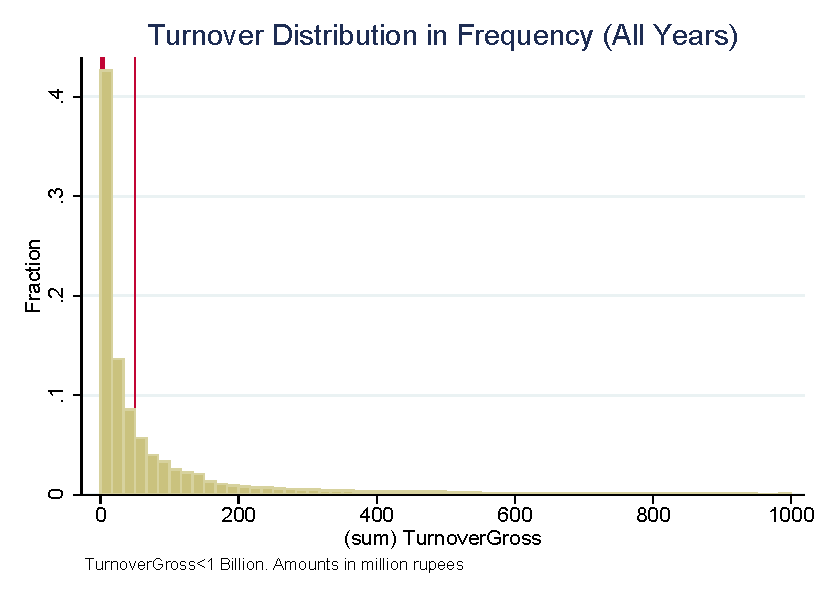
\includegraphics[width=1\textwidth]{graphs/TurnoverDistribution_Fraction_WeaklyPositive} 
\par\end{centering}
{\footnotesize{}{}{}Notes: }{\footnotesize \par}
\end{figure}

\newpage{}

\begin{figure}[t]
\caption{Firm Revenue Distribution at the Low Threshold}

\label{fig:LowestThreshold} 
\begin{centering}
\begin{tabular}{cc}
\vspace{0.2cm}
  & \vspace{0.2cm}
 \tabularnewline
\textbf{A: Bunching in Year 1}  & \textbf{B: Bunching in Year 2}\tabularnewline
b = 0.5  & b = 0.28\tabularnewline
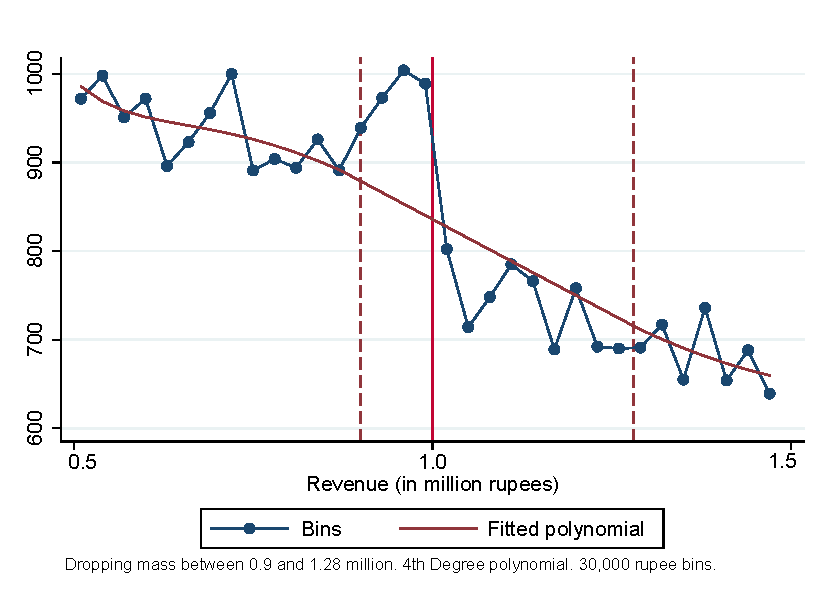
\includegraphics[width=0.4\textwidth]{graphs/BunchingYear1_1Million_Degree4_30000}  & 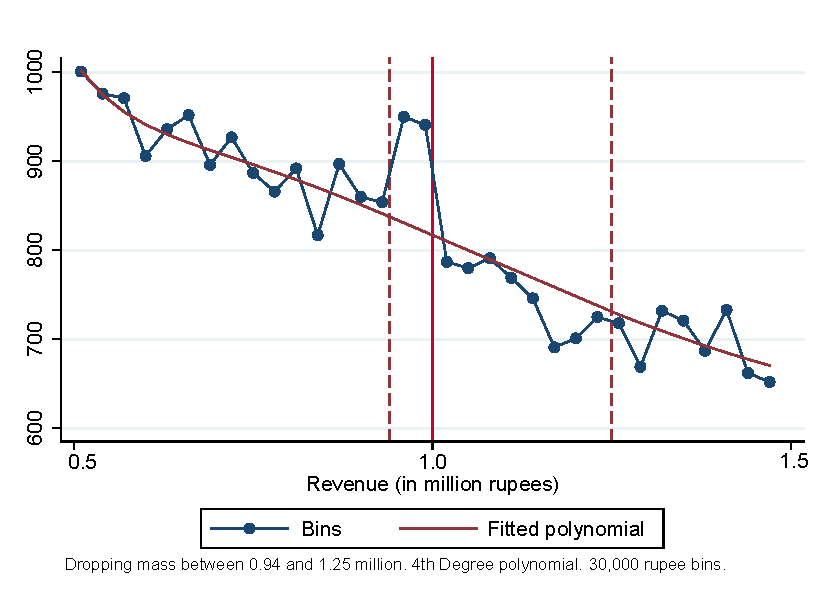
\includegraphics[width=0.4\textwidth]{graphs/BunchingYear2_1Million_Degree4_30000}\tabularnewline
\vspace{0.2cm}
  & \vspace{0.2cm}
 \tabularnewline
\textbf{C: No Bunching in Year 3}  & \textbf{D: No Bunching in Year 4}\tabularnewline
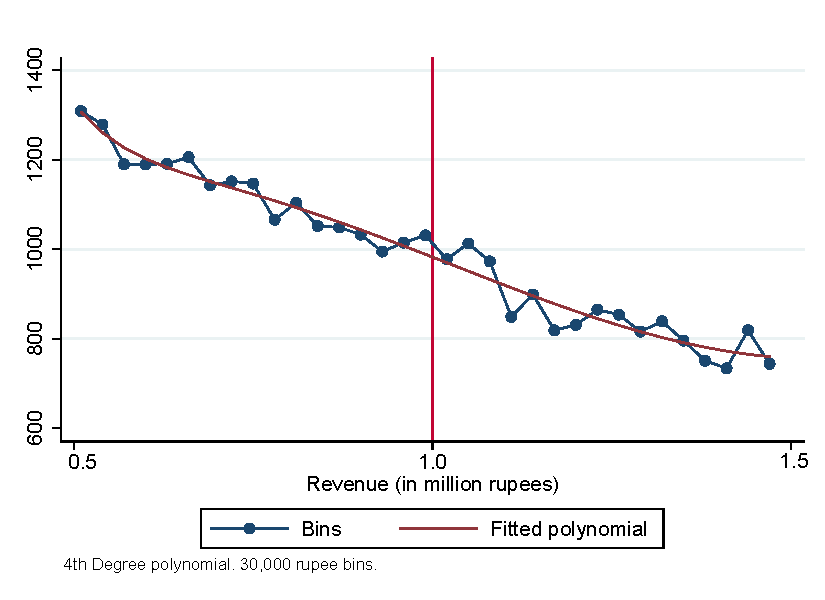
\includegraphics[width=0.4\textwidth]{graphs/BunchingYear3_1Million_Degree4_30000}  & 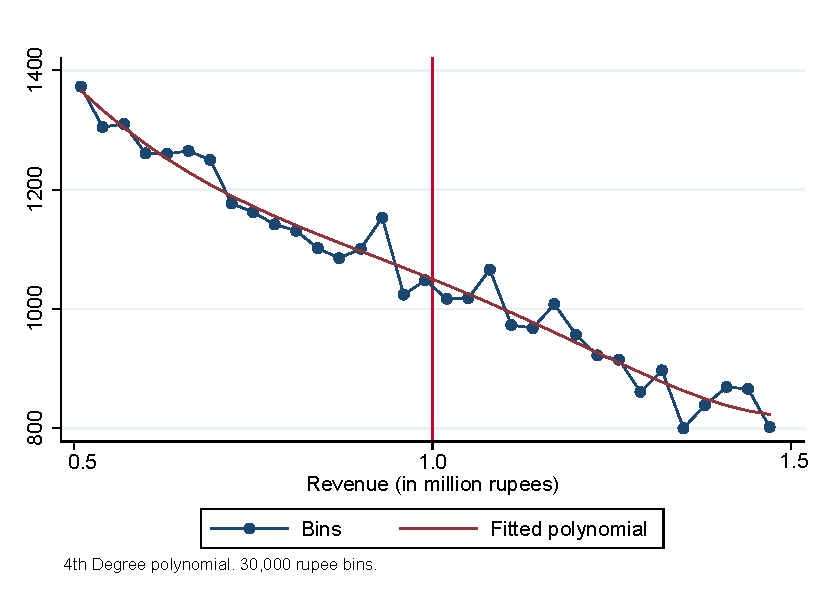
\includegraphics[width=0.4\textwidth]{graphs/BunchingYear4_1Million_Degree4_30000}\tabularnewline
\vspace{0.2cm}
  & \tabularnewline
\textbf{E: No Bunching in Year 5}  & \tabularnewline
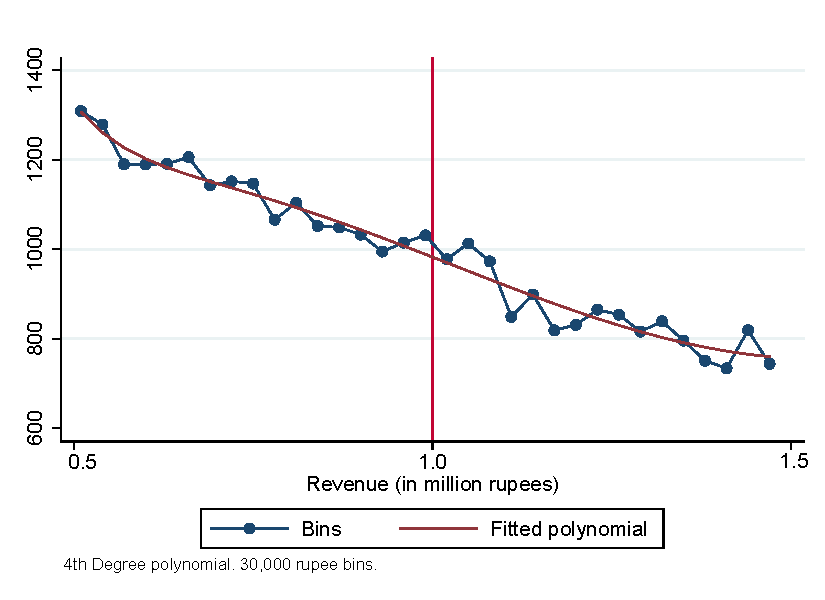
\includegraphics[width=0.4\textwidth]{graphs/BunchingYear3_1Million_Degree4_30000}  & \tabularnewline
\end{tabular}
\par\end{centering}
{\footnotesize{}{}{}Notes: }{\footnotesize \par}
\end{figure}

\newpage{}

\begin{figure}[t]
\caption{Firm Revenue Distribution at the Middle Threshold}

\label{fig:MiddleThreshold} 
\begin{centering}
\begin{tabular}{cc}
\vspace{0.2cm}
  & \vspace{0.2cm}
 \tabularnewline
\textbf{A: Bunching in Year 1}  & \textbf{B: Bunching in Year 2}\tabularnewline
b = 0.34  & b = 0.43\tabularnewline
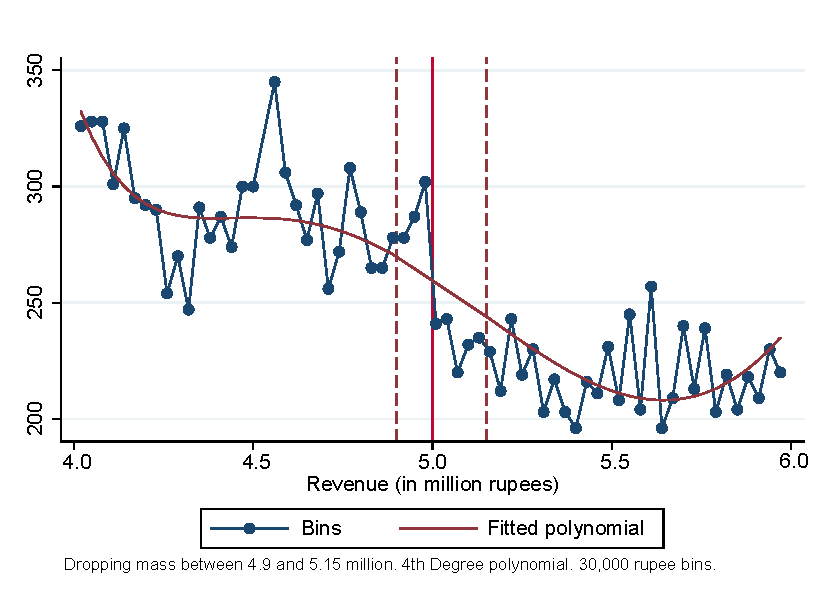
\includegraphics[width=0.4\textwidth]{graphs/BunchingYear1_5Million_Degree4_30000}  & 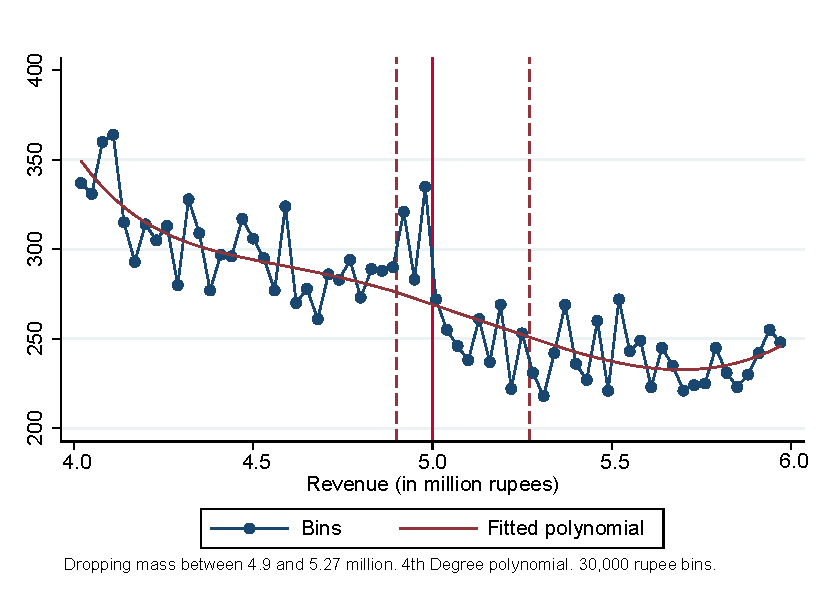
\includegraphics[width=0.4\textwidth]{graphs/BunchingYear2_5Million_Degree4_30000}\tabularnewline
\vspace{0.2cm}
  & \vspace{0.2cm}
 \tabularnewline
\textbf{C: No Bunching in Year 3}  & \textbf{D: No Bunching in Year 4}\tabularnewline
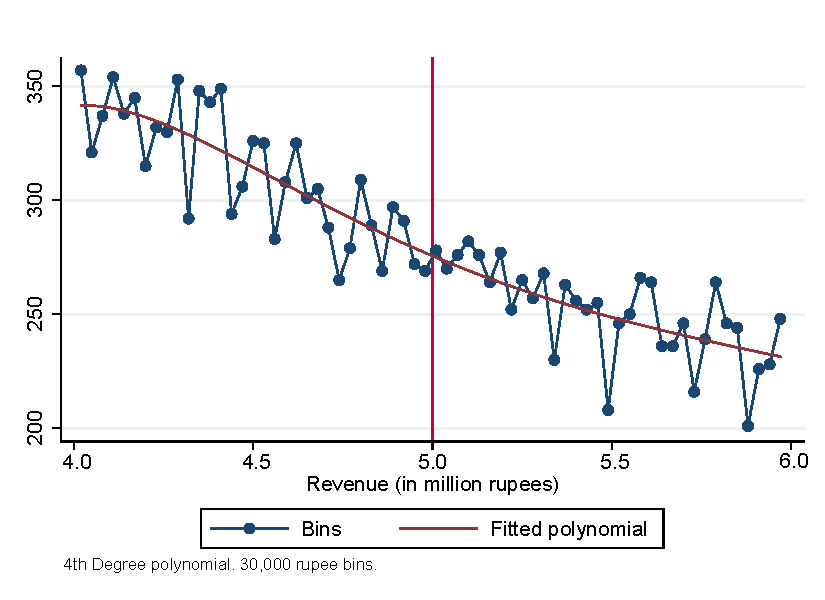
\includegraphics[width=0.4\textwidth]{graphs/BunchingYear3_5Million_Degree4_30000}  & 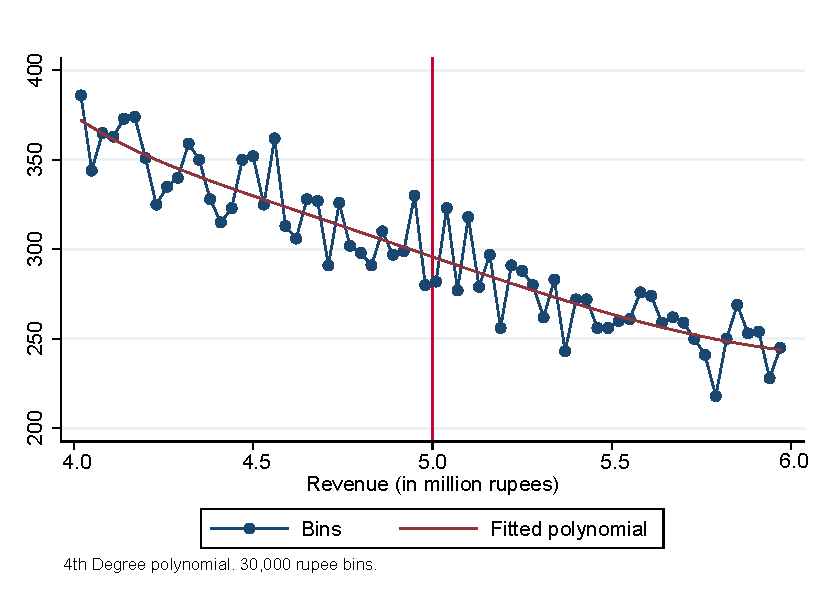
\includegraphics[width=0.4\textwidth]{graphs/BunchingYear4_5Million_Degree4_30000}\tabularnewline
\vspace{0.2cm}
  & \tabularnewline
\textbf{E: No Bunching in Year 5}  & \tabularnewline
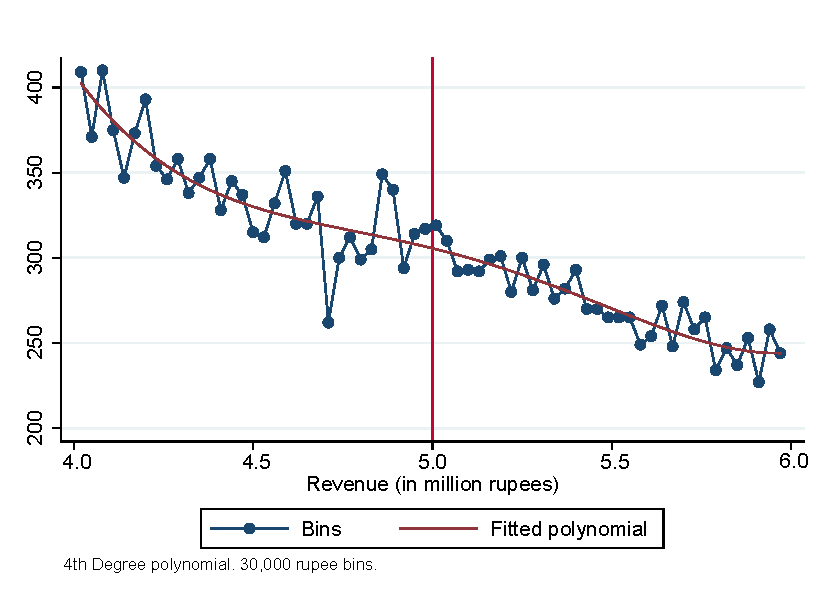
\includegraphics[width=0.4\textwidth]{graphs/BunchingYear5_5Million_Degree4_30000}  & \tabularnewline
\end{tabular}
\par\end{centering}
{\footnotesize{}{}{}Notes: }{\footnotesize \par}
\end{figure}

\newpage{}

\begin{figure}[t]
\caption{Firm Revenue Distribution at the High Threshold}

\label{fig:HighestThreshold} 
\begin{centering}
\begin{tabular}{cc}
\vspace{0.2cm}
  & \vspace{0.2cm}
 \tabularnewline
\textbf{A: Bunching in Year 1}  & \textbf{B: Bunching in Year 2}\tabularnewline
b = 2.6  & b = 2.98\tabularnewline
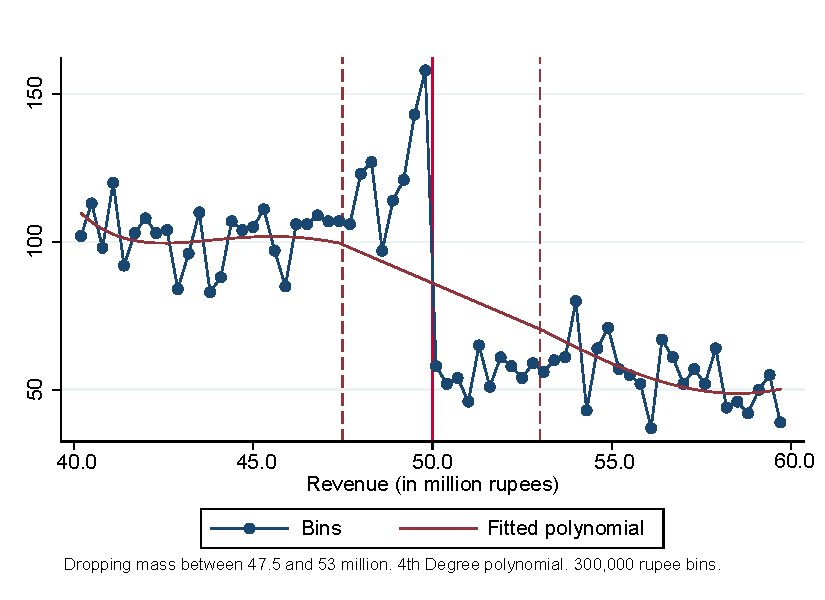
\includegraphics[width=0.4\textwidth]{graphs/BunchingYear1_50Million_Degree4_3lac}  & 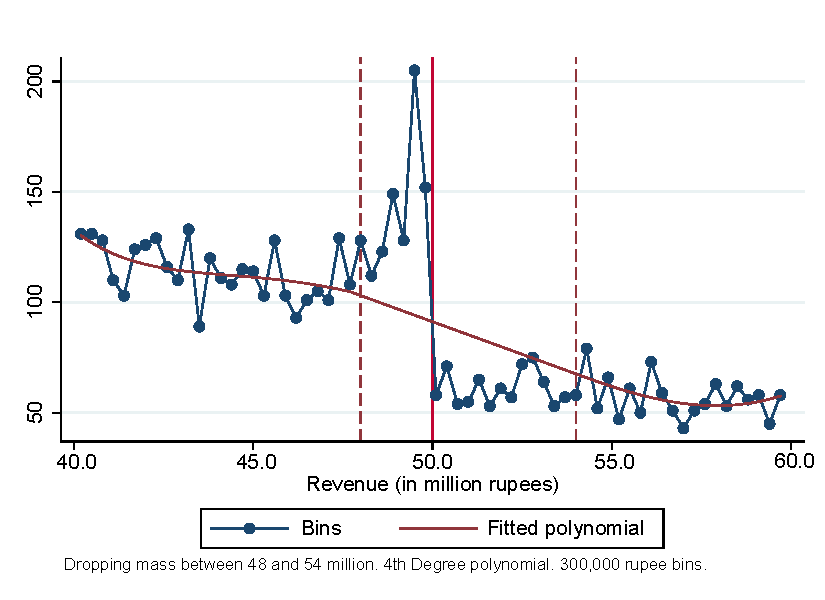
\includegraphics[width=0.4\textwidth]{graphs/BunchingYear2_50Million_Degree4_3lac}\tabularnewline
\vspace{0.2cm}
  & \vspace{0.2cm}
 \tabularnewline
\textbf{C: Bunching in Year 3}  & \textbf{D: No Bunching in Year 4}\tabularnewline
b = 1.87  & \tabularnewline
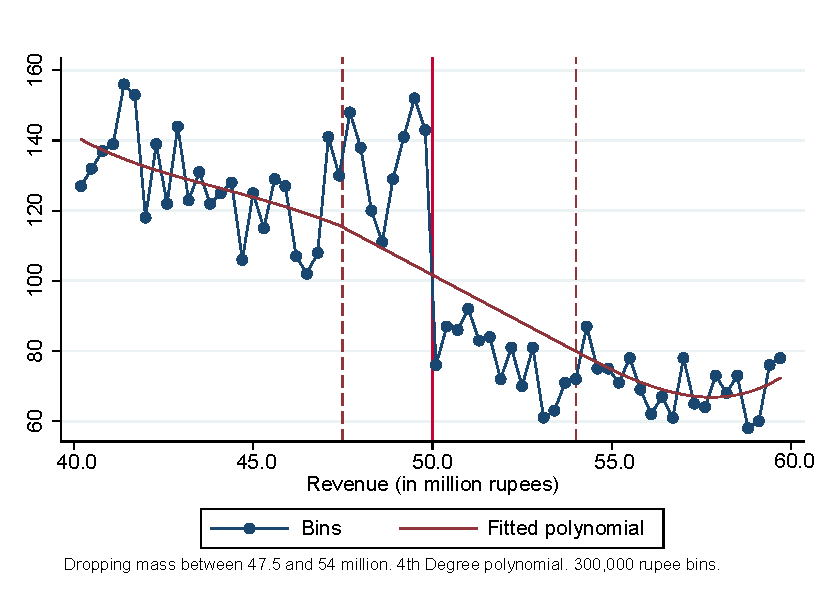
\includegraphics[width=0.4\textwidth]{graphs/BunchingYear3_50Million_Degree4_3lac}  & 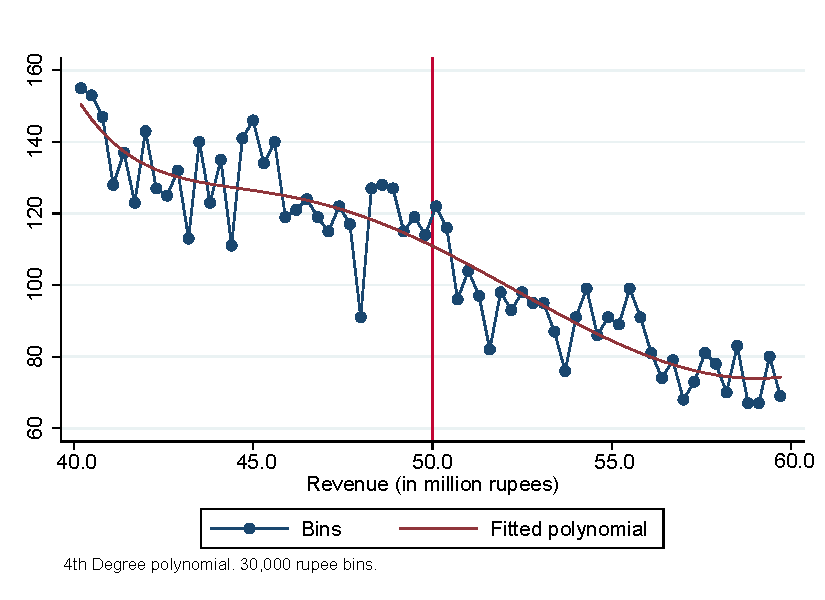
\includegraphics[width=0.4\textwidth]{graphs/BunchingYear4_50Million_Degree4_3lac}\tabularnewline
\vspace{0.2cm}
  & \tabularnewline
\textbf{E: No Bunching in Year 5}  & \tabularnewline
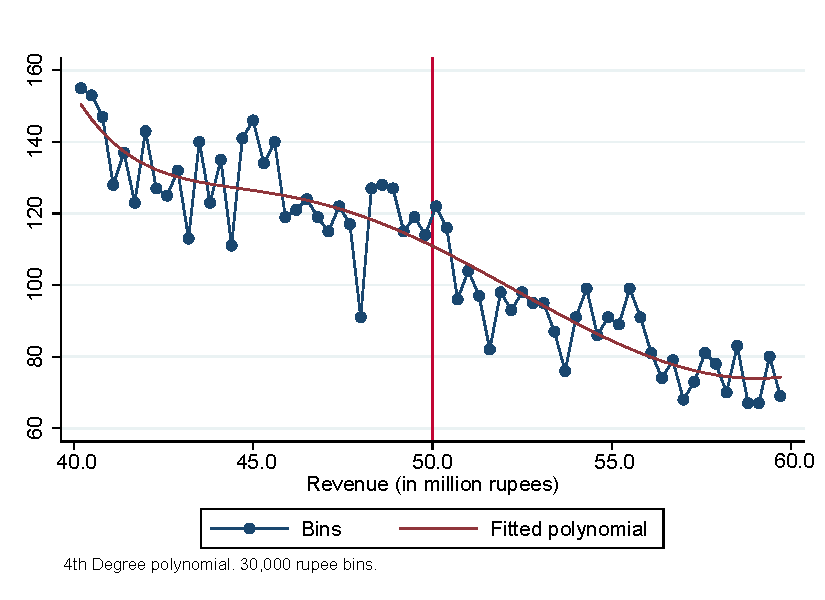
\includegraphics[width=0.4\textwidth]{graphs/BunchingYear4_50Million_Degree4_3lac}  & \tabularnewline
\end{tabular}
\par\end{centering}
{\footnotesize{}{}{}Notes: }{\footnotesize \par}
\end{figure}

\newpage{}

\begin{figure}[t]
\caption{Distribution of Compliance Costs by Revenue Size}

\label{fig:ComplianceCosts}\vspace{0.2cm}

\begin{centering}
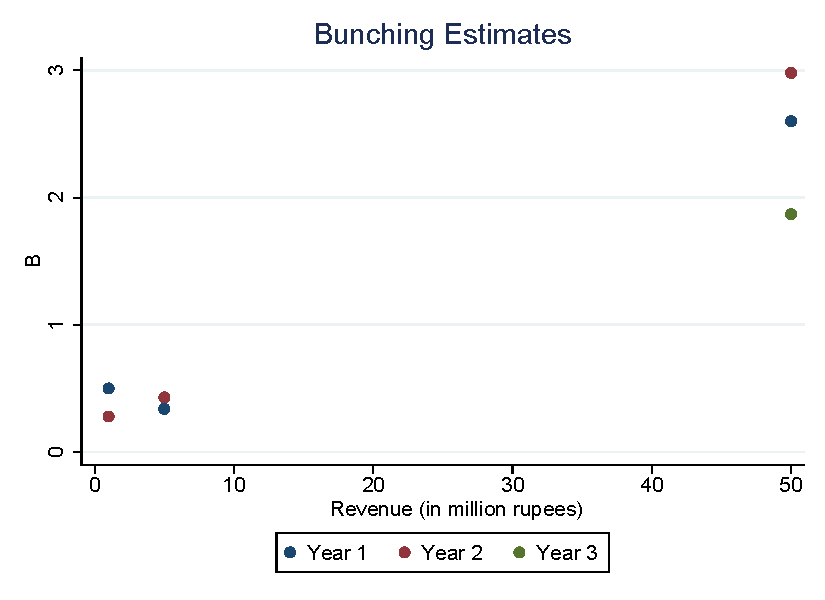
\includegraphics[width=1\textwidth]{graphs/BunchingEstimates} 
\par\end{centering}
{\footnotesize{}{}{}Notes: }{\footnotesize \par}
\end{figure}
